% Global Issues
% Compile with: latexmk -pdf global_issues.tex
\documentclass[aspectratio=169,11pt]{beamer}

\usepackage[T1]{fontenc}
\usepackage{lmodern}
\usepackage{booktabs}
\usepackage{array}
\usepackage{tikz}
\usetikzlibrary{shapes.geometric,positioning,calc,arrows.meta}
\usepackage{pgfplots}
\pgfplotsset{compat=1.18}
\usepackage[most]{tcolorbox}
\graphicspath{{images/}}

% ---------- Colors ----------
\definecolor{navy}{HTML}{1C2541}
\definecolor{oldred}{HTML}{B22234}   % US flag red, also the accent color
\definecolor{oldblue}{HTML}{3C3B6E}  % US flag blue
\definecolor{ink}{HTML}{2B2B2B}
\definecolor{muted}{HTML}{8A8F98}
\definecolor{paper}{HTML}{FFFFFF}
\definecolor{dem}{HTML}{2E5FA3}      % Democrats
\definecolor{rep}{HTML}{C0392B}      % Republicans
\definecolor{austria}{HTML}{C8102E}  % Austria red, for USA-vs-Austria comparisons

% ---------- Minimal theme ----------
\setbeamertemplate{navigation symbols}{}
\setbeamercolor{normal text}{fg=ink, bg=paper}
\setbeamercolor{structure}{fg=navy}
\setbeamercolor{frametitle}{fg=navy}
\setbeamercolor{alerted text}{fg=oldred}
\setbeamercolor{footnote}{fg=muted}
\setbeamerfont{frametitle}{size=\Large, series=\bfseries}
\setbeamertemplate{itemize item}{\color{oldred}\textbullet}
\setbeamertemplate{itemize subitem}{\color{muted}--}
\setbeamertemplate{enumerate item}{\color{oldred}\insertenumlabel.}
\setbeamersize{text margin left=1.1cm, text margin right=1.1cm}
\hypersetup{colorlinks=true, urlcolor=dem, linkcolor=navy}

\setbeamertemplate{frametitle}{%
  \vspace*{0.5cm}%
  \usebeamerfont{frametitle}\usebeamercolor[fg]{frametitle}\insertframetitle\par
  \vspace{0.15cm}{\color{navy!15}\rule{\textwidth}{0.4pt}}\par}

\setbeamertemplate{footline}{%
  \hfill{\tiny\color{muted}\insertframenumber}\hspace*{0.6cm}\vspace*{0.35cm}}

% Plain divider at the start of each section
\AtBeginSection{%
  \begin{frame}[plain,noframenumbering]
    \centering
    {\LARGE\bfseries\color{navy}\insertsection}\\[0.6em]
    {\color{oldred}\rule{1.5cm}{0.8pt}}
  \end{frame}}

% "Think" question slides: \begin{thinkframe} ... \end{thinkframe}
\newenvironment{thinkframe}{%
  \begin{frame}[plain,noframenumbering,environment=thinkframe]\centering\Large}{\end{frame}}

% ---------- Helpers ----------
% Small grey source line at the bottom of a frame
\newcommand{\source}[1]{%
  \begin{tikzpicture}[remember picture,overlay]
    \node[anchor=south west, font=\tiny, text=muted, text width=0.85\paperwidth, align=left]
      at ($(current page.south west)+(0.6cm,0.25cm)$) {#1};
  \end{tikzpicture}}

% Quote box with a thin red rule on the left; optional arg e.g. [fontupper=\itshape\small]
\newtcolorbox{textquote}[1][]{%
  enhanced, frame hidden, boxrule=0pt, sharp corners,
  colback=navy!4, borderline west={2pt}{0pt}{oldred},
  left=10pt, right=8pt, top=6pt, bottom=6pt, fontupper=\itshape, #1}

% Photo + name + short bio (use inside a column): \candidate{file}{Name}{bio}
\newcommand{\candidate}[3]{%
  \begin{minipage}[t]{\linewidth}\centering
    \includegraphics[height=3.5cm]{#1}\\[0.5em]
    {\large\bfseries\color{navy}#2}\\[0.4em]
    \begin{minipage}{0.9\linewidth}\raggedright\small #3\end{minipage}
  \end{minipage}}

% Big number with a caption (use inside a column): \bignum{color}{91\%}{caption}
\newcommand{\bignum}[3]{%
  \begin{minipage}[t]{\linewidth}\centering
    {\fontsize{34}{38}\selectfont\bfseries\color{#1}#2}\\[0.3em]
    {\small #3}
  \end{minipage}}

% US flag drawn in TikZ (hoist height = #1), e.g. \usflag{3cm}
\newcommand{\usflag}[1]{%
  \begin{tikzpicture}[x=#1, y=#1]
    \def\fly{1.9}
    \foreach \i in {0,...,12} {
      \pgfmathsetmacro{\c}{mod(\i,2)==0 ? 1 : 0}
      \ifdim\c pt=1pt
        \fill[oldred] (0,{1-(\i+1)/13}) rectangle (\fly,{1-\i/13});
      \else
        \fill[white] (0,{1-(\i+1)/13}) rectangle (\fly,{1-\i/13});
      \fi
    }
    \def\cw{0.76} \def\ch{0.5385}
    \fill[oldblue] (0,{1-\ch}) rectangle (\cw,1);
    \foreach \r in {1,...,9} {
      \pgfmathsetmacro{\isodd}{mod(\r,2)}
      \ifdim\isodd pt=1pt
        \foreach \k in {0,...,5}
          \node[star, star points=5, star point ratio=2.618, fill=white, inner sep=0pt,
                minimum size=0.0616*#1] at ({(2*\k+1)*\cw/12},{1-\r*\ch/10}) {};
      \else
        \foreach \k in {0,...,4}
          \node[star, star points=5, star point ratio=2.618, fill=white, inner sep=0pt,
                minimum size=0.0616*#1] at ({(2*\k+2)*\cw/12},{1-\r*\ch/10}) {};
      \fi
    }
    \draw[ink!30, line width=0.3pt] (0,0) rectangle (\fly,1);
  \end{tikzpicture}}

% Agree/disagree spectrum for "spectrum game" activities
\newcommand{\spectrum}{%
  
\begin{tikzpicture}
    \shade[left color=oldblue, right color=oldred, rounded corners=2pt] (0,0) rectangle (11,0.18);
    \node[anchor=north, font=\small, text=oldblue] at (0,-0.15) {Strongly disagree};
    \node[anchor=north, font=\small, text=muted] at (5.5,-0.15) {Neutral};
    \node[anchor=north, font=\small, text=oldred] at (11,-0.15) {Strongly agree};
    \fill[paper, draw=muted] (5.5,0.09) circle (2.5pt);
  \end{tikzpicture}}

% One statement per slide: \statement{number}{total}{text}
\newcommand{\statement}[3]{%
  \begin{frame}[plain]
    \vfill
    \begin{center}
      {\small\color{muted}Statement #1 of #2}\\[1.2em]
      {\LARGE\bfseries #3}
    \end{center}
    \vfill
    \begin{center}\spectrum\end{center}
    \vspace{1.2cm}
  \end{frame}}

% Large red initial for the MPOWER slide
\newcommand{\mpl}[1]{{\LARGE\bfseries\color{oldred}#1}}

\begin{document}

% ---------- Title slide ----------
\begin{frame}[plain]
  \begin{columns}[c]
    \begin{column}{0.55\textwidth}
      {\fontsize{30}{34}\selectfont\bfseries\color{navy} Global\\Issues}\\[0.8em]
      {\Large\color{muted} Who is in charge when a problem crosses borders?}\\[0.6em]
      {\color{oldred}\rule{3cm}{1.5pt}}
    \end{column}
    \begin{column}{0.4\textwidth}
      \centering
      
\includegraphics[width=\linewidth]{unflag.png}
    \end{column}
  \end{columns}
\end{frame}

% =====================================================================
\section{Warm-up}

\begin{frame}{Warm-up}
  Which of these global issues are regulated by an \alert{international organization}?
  \vspace{0.8em}
  \begin{columns}[T]
    \begin{column}{0.42\textwidth}
      \begin{itemize}\setlength{\itemsep}{0.9em}
        \item Pandemics
        \item Air travel
        \item The internet
      \end{itemize}
    \end{column}
    \begin{column}{0.42\textwidth}
      \begin{itemize}\setlength{\itemsep}{0.9em}
        \item Mail
        \item Nuclear technology
        \item Artificial intelligence
      \end{itemize}
    \end{column}
  \end{columns}
\end{frame}

\begin{frame}{Five out of six}
  \centering
  \renewcommand{\arraystretch}{1.45}
  \begin{tabular}{@{}l@{\hspace{1.2cm}}c@{\hspace{1.2cm}}l@{}}
    Pandemics & $\rightarrow$ & \textbf{\color{navy}WHO} \\
    Air travel & $\rightarrow$ & \textbf{\color{navy}ICAO} \\
    The internet & $\rightarrow$ & \textbf{\color{navy}ITU} {\small\color{muted}(partly)} \\
    Mail & $\rightarrow$ & \textbf{\color{navy}UPU} \\
    Nuclear technology & $\rightarrow$ & \textbf{\color{navy}IAEA} \\
    Artificial intelligence & $\rightarrow$ & \textbf{\color{oldred}?} \\
  \end{tabular}

  \vspace{1em}
  {\small All five are part of the \alert{United Nations} system\par}
\end{frame}

\begin{frame}{What is a UN specialized agency?}
  \begin{itemize}\setlength{\itemsep}{0.9em}
    \item An independent organization linked to the UN by treaty
    \item Its own members, budget and leadership
    \item Countries \alert{choose} to join, and can leave
    \item It sets shared rules, but has \alert{no police and no army}: it depends on countries to follow them
  \end{itemize}
\end{frame}

% =====================================================================
\section{Pandemics}

\begin{frame}{The problem: pandemics}
  \begin{itemize}\setlength{\itemsep}{0.9em}
    \item A virus does not stop at a border
    \item COVID-19 reached almost every country within \alert{three months}
    \item More than \alert{7 million} reported deaths worldwide
    \item What happens if every country keeps its data to itself?
  \end{itemize}
  \source{Source: WHO COVID-19 dashboard.}
\end{frame}

\begin{frame}{World Health Organization (WHO)}
  \begin{itemize}\setlength{\itemsep}{0.7em}
    \item \textbf{Headquarters:} Geneva, Switzerland
    \item \textbf{Founded:} 7 April 1948 (now World Health Day)
    \item \textbf{Members:} 194 countries
    \item \textbf{Goal:} ``the attainment by all peoples of the highest possible level of health''
    \item \textbf{US connection:} the US announced its withdrawal in January 2025 and says it left in January 2026
  \end{itemize}
  \source{Source: WHO Constitution, Article 1; HHS, Jan.\ 2026.}
\end{frame}

\begin{frame}{What does that mean?}
  \begin{itemize}\setlength{\itemsep}{0.9em}
    \item \alert{Coordinates the global response} to outbreaks: collects data, declares emergencies, issues guidance
    \item \alert{Sets health standards} that countries can adopt
      \begin{itemize}
        \item Example (2025): ``use of lower-sodium salt substitutes''
      \end{itemize}
    \item \alert{Runs long-term campaigns}, such as \textbf{MPOWER} against tobacco
  \end{itemize}
  \source{Source: WHO, \emph{Use of lower-sodium salt substitutes} (Jan.\ 2025).}
\end{frame}

\begin{frame}{MPOWER: six steps against tobacco}
  \renewcommand{\arraystretch}{1.5}
  \begin{tabular}{@{\hspace{0.6cm}}c@{\hspace{0.5cm}}l@{}}
    \mpl{M} & \textbf{Monitor} tobacco use and prevention policies \\
    \mpl{P} & \textbf{Protect} people from tobacco smoke \\
    \mpl{O} & \textbf{Offer} help to quit tobacco use \\
    \mpl{W} & \textbf{Warn} about the dangers of tobacco \\
    \mpl{E} & \textbf{Enforce} bans on tobacco advertising, promotion and sponsorship \\
    \mpl{R} & \textbf{Raise} taxes on tobacco \\
  \end{tabular}
  \source{Source: WHO, MPOWER (introduced 2008).}
\end{frame}

% =====================================================================
\section{Air Travel}

\begin{frame}{The problem: air travel}
  \small
  \begin{itemize}\setlength{\itemsep}{0.25em}
    \item More than \alert{100,000 flights} take off every day
    \item A plane built in the US, flown by an Austrian airline, lands in Japan. On the way it crosses about \alert{ten countries}
    \item Which country's rules apply? What language does the pilot speak to the tower?
  \end{itemize}
  \vspace{0.2em}
  \centering
  % map covers lon 0..150 (x) and lat 15..62 (y): x = lon/150*W, y = (lat-15)/47*H
  \begin{tikzpicture}[x=9.6cm/150, y=3.0cm/47]
    \node[anchor=south west, inner sep=0pt] at (0,0) {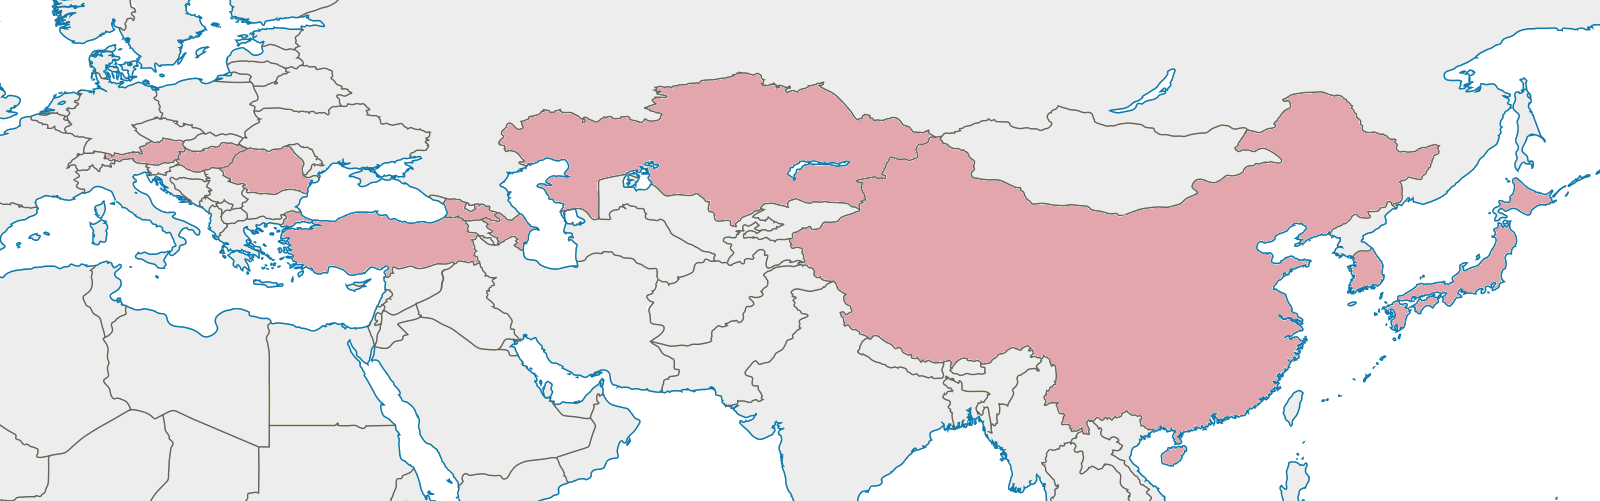
\includegraphics[width=9.6cm,height=3.0cm]{routemap.png}};
    \draw[oldred, line width=1.3pt, line cap=round]
      plot[smooth, tension=0.6] coordinates {
        (16.6,33.1) (21,31.6) (27.5,29.6) (35,26.8) (43,26.7) (49,25.6) (52,27.6)
        (60,31.3) (69,30) (80,29.3) (95,27) (110,25) (120,23.3) (127,22.3) (135,21.2) (140.4,20.8)};
    \fill[navy] (16.6,33.1) circle (2.2pt);
    \fill[navy] (140.4,20.8) circle (2.2pt);
    \node[font=\scriptsize\bfseries, text=navy, anchor=south] at (16.6,34) {Vienna};
    \node[font=\scriptsize\bfseries, text=navy, anchor=north west] at (140.4,20.3) {Tokyo};
  \end{tikzpicture}\\[0.2em]
  {\tiny\color{ink} Austria $\rightarrow$ Hungary $\rightarrow$ Romania $\rightarrow$ Turkey $\rightarrow$ Georgia $\rightarrow$ Azerbaijan $\rightarrow$ Kazakhstan $\rightarrow$ China $\rightarrow$ South Korea $\rightarrow$ Japan\par}
  \source{Source: ICAO; Austrian Airlines. Typical route, varies daily. Map: TUBS, CC BY-SA 3.0 (modified).}
\end{frame}

\begin{frame}{International Civil Aviation Organization (ICAO)}
  \begin{itemize}\setlength{\itemsep}{0.8em}
    \item \textbf{Headquarters:} Montreal, Canada
    \item \textbf{Founded:} 4 April 1947
    \item \textbf{Members:} 193 countries
    \item \textbf{What it does:} sets shared standards for safety, pilot licences, airports and air traffic rules
    \item \textbf{US connection:} created by the Chicago Convention, signed in Chicago in 1944
  \end{itemize}
  \source{Source: ICAO.}
\end{frame}

\begin{frame}{ICAO standards you have already met}
  \begin{itemize}\setlength{\itemsep}{0.7em}
    \item \alert{English:} every pilot and controller on international flights must pass an English test (ICAO ``Level 4'')
    \item \alert{The alphabet:} Alfa, Bravo, Charlie \ldots\ so that ``B'' and ``D'' are never confused over the radio
    \item \alert{Your passport:} the same size in every country, with two lines of machine-readable code at the bottom
    \item \alert{Black boxes:} every airliner must carry flight recorders, and crash reports are shared with all countries
    \item \alert{Airport codes:} Vienna is \textbf{LOWW} to every pilot in the world
  \end{itemize}
\end{frame}

\begin{frame}{What if a country doesn't follow the rules?}
  \begin{itemize}\setlength{\itemsep}{0.9em}
    \item ICAO has \alert{no power to punish} anyone. It can only inspect and publish the results
    \item But other countries can \alert{close their airspace} to airlines they don't trust
    \item Example: in 2020, Pakistan found that almost a third of its pilots had fake or suspicious licences
    \item The EU \alert{banned} Pakistan's national airline for more than four years (2020--2024)
  \end{itemize}
  \source{Source: EASA, Nov.\ 2024.}
\end{frame}

% =====================================================================
\section{The Internet}

\begin{frame}{The problem: staying connected}
  \begin{itemize}\setlength{\itemsep}{0.9em}
    \item Radio signals and satellites ignore borders
    \item Your phone works when you land in another country
    \item Every country has its own calling code: \alert{+43} Austria, \alert{+1} USA
    \item Who decides who gets which frequency, and which number?
  \end{itemize}
\end{frame}

\begin{frame}{International Telecommunication Union (ITU)}
  \begin{itemize}\setlength{\itemsep}{0.7em}
    \item \textbf{Headquarters:} Geneva, Switzerland
    \item \textbf{Founded:} 17 May 1865, as the International \emph{Telegraph} Union: the oldest UN agency
    \item \textbf{Members:} 194 countries
    \item \textbf{What it does:} divides up radio frequencies and satellite orbits, sets technical standards, assigns country calling codes
    \item \textbf{US connection:} its Secretary-General, Doreen Bogdan-Martin, is American
  \end{itemize}
  \source{Source: ITU.}
\end{frame}

\begin{frame}{The ITU in practice}
  \begin{itemize}\setlength{\itemsep}{0.8em}
    \item Your laptop finds Wi-Fi in Vienna, New York and Tokyo, because Wi-Fi uses the \alert{same frequencies} everywhere
    \item A radio station in Vienna and one in Bratislava (60 km away) don't drown each other out
    \item Every satellite, including Starlink's, has to be \alert{registered} with the ITU
    \item \textbf{But:} it does \emph{not} run the internet. Web addresses are managed by \alert{ICANN}, a non-profit based in California
  \end{itemize}
  \source{Source: ITU; ICANN.}
\end{frame}

% =====================================================================
\section{Mail}

\begin{frame}{The problem: sending a letter abroad}
  \begin{itemize}\setlength{\itemsep}{0.9em}
    \item You buy an Austrian stamp and post a letter to New York
    \item The Austrian post gets your money. The \alert{US} post does the delivery
    \item Before 1874: a separate treaty between every pair of countries, and a different price for every route
    \item Who pays the American mail carrier?
  \end{itemize}
\end{frame}

\begin{frame}{Universal Postal Union (UPU)}
  \small
  \begin{itemize}\setlength{\itemsep}{0.3em}
    \item \textbf{Headquarters:} Bern, Switzerland
    \item \textbf{Founded:} 9 October 1874 (now World Post Day)
    \item \textbf{Members:} 192 countries
    \item \textbf{What it does:} makes the world ``a single postal territory.'' Three rules:
      \begin{itemize}\setlength{\itemsep}{0.2em}
        \item \alert{Deliver it like your own:} every member must deliver foreign mail as if it were domestic mail
        \item \alert{Freedom of transit:} every member must pass on mail that is only travelling through
        \item \alert{Terminal dues:} the sending country pays the delivering country a fixed fee, set by the UPU
      \end{itemize}
    \item \textbf{US connection:} in 2018 the US announced it would leave, saying the fees made it too cheap to ship parcels from China. It stayed after the rules were changed in 2019
  \end{itemize}
  \source{Source: UPU Constitution, Article 1; Universal Postal Convention.}
\end{frame}

% =====================================================================
\section{Nuclear Technology}

\begin{frame}{The problem: nuclear technology}
  \begin{itemize}\setlength{\itemsep}{0.9em}
    \item The same technology makes \alert{electricity} and \alert{bombs}
    \item \alert{Nine} countries have nuclear weapons: about \alert{12,000} warheads
    \item A country says its nuclear program is only for energy. How does anyone know?
  \end{itemize}
  \source{Source: SIPRI Yearbook 2025.}
\end{frame}

\begin{frame}{International Atomic Energy Agency (IAEA)}
  \begin{columns}[c]
    \begin{column}{0.58\textwidth}
      \small
      \begin{itemize}\setlength{\itemsep}{0.35em}
        \item \textbf{Headquarters:} \alert{Vienna}, Austria
        \item \textbf{Founded:} 29 July 1957
        \item \textbf{Members:} about 180 countries
        \item \textbf{What it does:} helps countries use nuclear technology peacefully, and sends \alert{inspectors} to check that it stays peaceful
        \item Nobel Peace Prize, 2005
        \item \textbf{US connection:} proposed by President Eisenhower in his ``Atoms for Peace'' speech at the UN, 1953
      \end{itemize}
      \vspace{0.4em}
    \end{column}
    \begin{column}{0.38\textwidth}
      \centering
      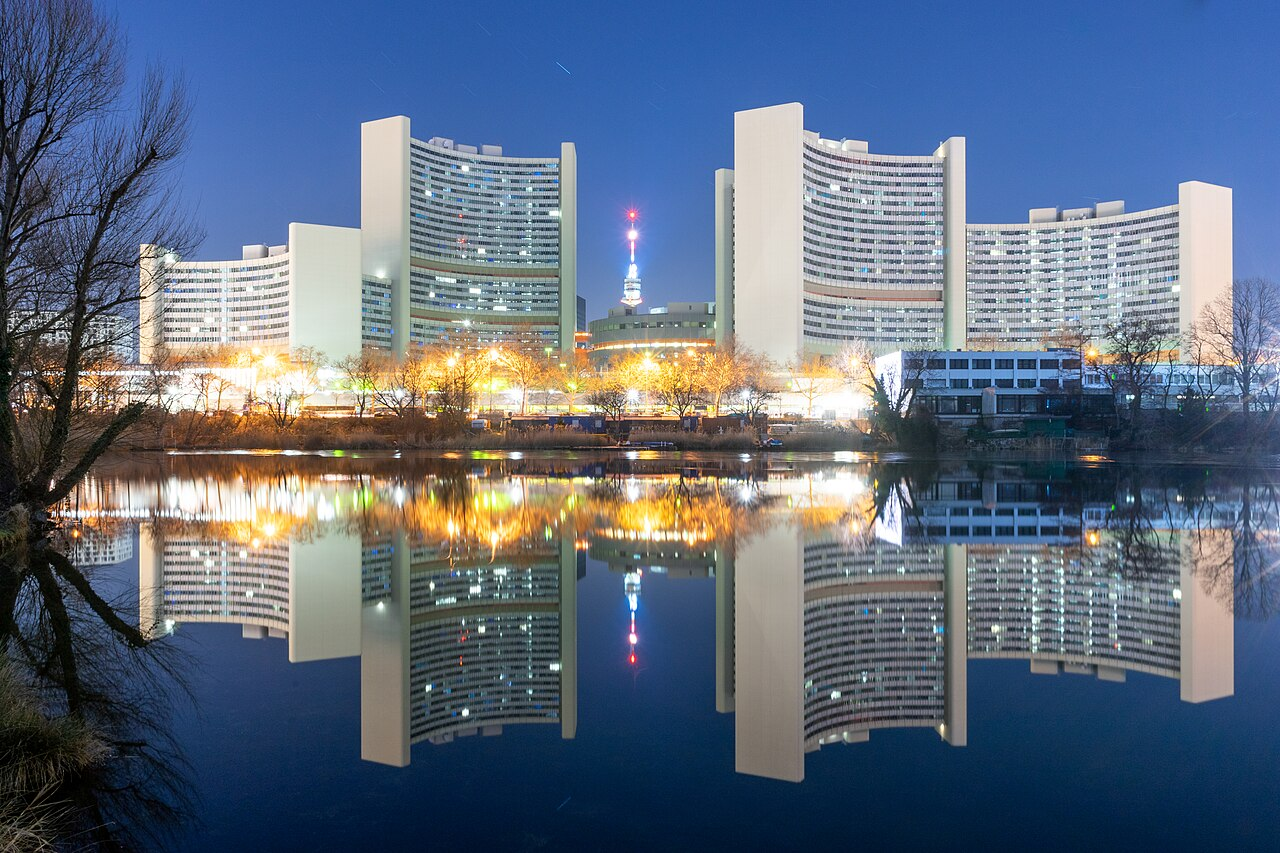
\includegraphics[width=\linewidth]{vic2.jpg}\\[0.2em]
      {\tiny\color{muted} Vienna International Centre (``UNO City''). Photo: Dimitry Anikin, CC0\par}
    \end{column}
  \end{columns}
  \source{Source: IAEA.}
\end{frame}

% =====================================================================
\section{Artificial Intelligence}

\begin{frame}{The problem: artificial intelligence}
  \begin{itemize}\setlength{\itemsep}{0.9em}
    \item Built by a handful of companies, mostly in the \alert{US} and \alert{China}
    \item Used in almost every country
    \item Rules so far are a patchwork: the EU has its \alert{AI Act} (2024); most countries have little or nothing
    \item New risks keep appearing: \alert{deepfakes}, AI-designed \alert{bioweapons}, \ldots
  \end{itemize}
\end{frame}

\begin{frame}{Create your own agency}
  \begin{itemize}\setlength{\itemsep}{1em}
    \item \textbf{Should there be a ``WHO for AI''?}
    \item Which of today's organizations would be the best model?
    \item Would the US and China join?
  \end{itemize}
\end{frame}

\end{document}
